\begin{frame}
  \frametitle{Tableaux Calculus}
  {\bf Question:} How do we formally show that there is no model?
  \pause
  \bigskip
  We use a formal proof system:\\
  The tableaux calculus (as in \cite{gore07}). \\
  We have four rules:
  \[
  (\bot) \, \Gamma: \frac{X; A; \lnot A}{\bot}, \quad
  (\sqcap) \, \Gamma: \frac{X; C \sqcap D}{X; C; D}, \quad
  (\sqcup) \, \Gamma: \frac{X; C \sqcup D}{X; C | X; D},
  \]
  \[
  (\exists R) \, \Gamma: \frac{X; \exists R. C}{\{D | \forall R.D \in X\};  C ; \Gamma}.
  \]
  \pause
  We have a proof if we can \emph{close} all the branches with a $\bot$.
  \pause
  This proof system is sound \& complete with respect to $\mathcal{ALC}$.
\end{frame}

\begin{frame}
  \frametitle{The Program: Structure}
  \begin{figure}
  \begin{center}
    \includegraphics[scale=0.2]{design.jpeg}
  \end{center}
\end{figure}
\end{frame}

\begin{frame}
  \frametitle{The Program: Main Components}
\textbf{Parser.} Automatically generated from a grammar. \\
\vspace{1cm}\pause
\textbf{Proof/Model Search.} Gets a knowledgebase and a set of concepts. Generates either
a proof or model. \\
\vspace{1cm}\pause
\textbf{Proof Checker.} Checks if a proof is correct. If not, gives helpful advice. \\
\vspace{1cm}\pause
\textbf{Model Checker.} Checks if a model is correct. If not, gives helpful advice. \\
\end{frame}
